\chapter{関連研究}
\section{グラフ構造}
\subsection{グラフ構造の表現}
グラフはノードと2つのノード同士を結ぶエッジから構成されている。つまりノードの集合を$\mathcal{V}$、エッジの集合を$\mathcal{E}$とすると、グラフ$\mathcal{G}$は$\mathcal{G} = (\mathcal{V},\mathcal{E})$と表せる。グラフの種類としては、エッジに向きが存在する有向グラフ、同じノードペアに多重のエッジが張られるグラフ、セルフループというノードから同じノードにエッジが張られるグラフや、エッジごとに重みがあるグラフなど様々な種類が存在するが、本研究ではセルフループなしの無向重みなしグラフを用いる。そのようなグラフは隣接行列$\mathbf{A} \in R^{N \times N}$を用いて表現することができる。ここでノード$v_i,v_j$間にエッジが存在する場合、つまり$(v_{i},v_{j}) \in \mathcal{E}$のときには$A_{ij} = 1$として表現する。一方でノード$v_i,v_j$間にエッジが存在しない場合、つまり$(v_{i},v_{j}) \notin \mathcal{E}$のときには$A_{ij} = 0$として表す。図\ref{fig:graph}はグラフ構造の例である。この例の左図ではノード数6、エッジ数5のグラフを視覚的に示しており、そのグラフ構造を右図では隣接行列を用いて示している。

\begin{figure*}[tb]
  \centering
  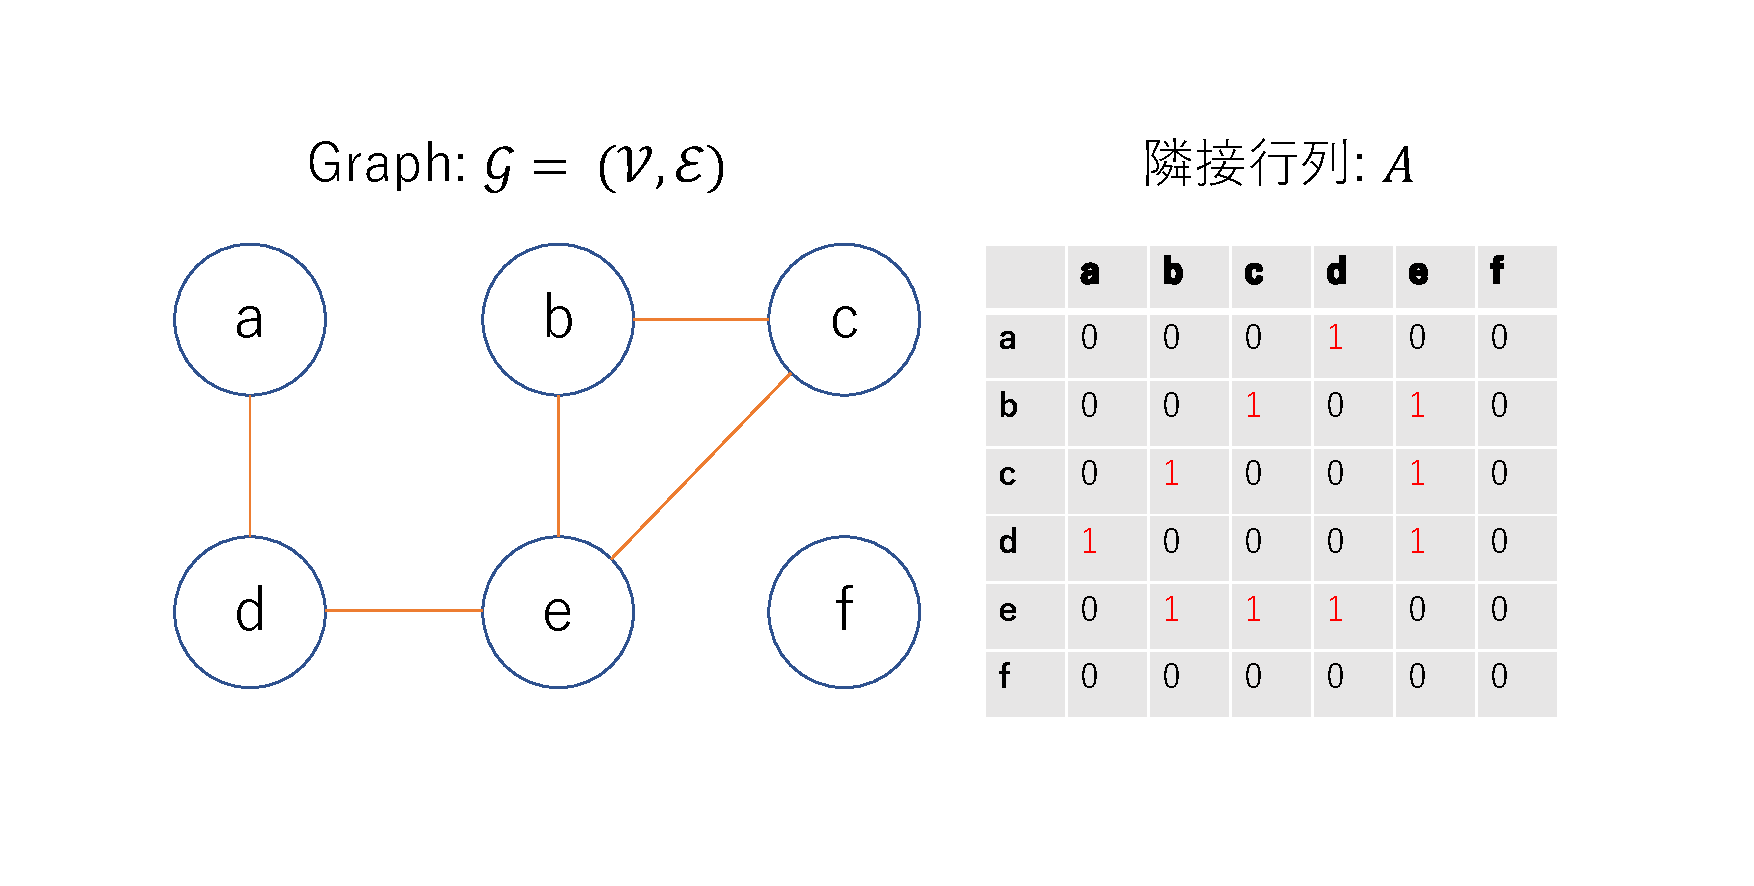
\includegraphics[width=0.8\hsize]{figures/graph_structure.pdf}
  \caption{グラフ表現の例}
  \label{fig:graph}
\end{figure*}

\subsection{グラフ構造を用いたタスク}
Getoor\cite{getoor2005link}やHamilton\cite{hamilton2020graph}によるとグラフ構造を用いたタスクは以下のようなものがある。
\begin{itemize}
\item ノードごとのタスク
	\begin{itemize}
	\item ノードの分類
	\item ノードのクラスタリング
	\item ノードのランキング
    \item ノードの特定
	\end{itemize}
\item エッジごとのタスク
	\begin{itemize}
	\item リンク予測
	\end{itemize}
\item グラフ全体によるタスク
	\begin{itemize}
    \item 部分グラフの特定
    \item グラフ分類
    \item グラフ生成モデルの作成
	\end{itemize}
\end{itemize}

近年のグラフ構造を用いた研究の関心の高まりにより、これらのどのタスクにおいても近年多くの研究がされている。本研究ではこの中でもノード分類とリンク予測についてに注目し研究対象とした。


\section{半教師ありノード分類}
ノード分類はグラフ構造や特徴量からノードのラベルを予測するタスクである。その中でも半教師ありノード分類は、グラフ全体の構造、それぞれのノードにおける特徴量、少数のノードのラベルを用い、ラベルが与えられていない残りのノードのラベル予測をするタスクである。

グラフを$\mathcal{G}=(\mathcal{V},\mathcal{E})$、ノード数を$n = |\mathcal{V}|$とすると隣接行列は$\mathbf{A} \in R^{n\times n}$となる。特徴量行列の集合を$\mathbf{X} = \{\boldsymbol{x_{1}},..., \boldsymbol{x_{n}}\}$、用いるラベルの個数を$l$とし、ノードの集合を$\mathcal{V} = \{ v_{1}, . . . , v_{l}, v_{l+1}, . . . , v_{n}\}$とする。またそれぞれのノードにおけるラベルをそれぞれ$y_{1}, ..., y_{n}$とする。これらにより、半教師あり分類問題は以下のように定義される。

\begin{itemize}
\item 入力:\\
隣接行列:$\mathbf{A} \in R^{n\times n}$,\\
全ノードの特徴ベクトル:$\mathbf{X}=\{\boldsymbol{x_{1}}, ..., \boldsymbol{x_{n}}\}$,\\
$l$個の教師ありラベル: $y_{1}, ...., y_{l}$
\item 出力:\\
$n-l$個の教師なしラベル: $y_{l+1}, ..., y_{n}$
\end{itemize}

半教師あり学習のタスクににおける重要な特徴の1つは、学習においてクラスラベルは一部の教師データのみを扱うが、グラフ構造と特徴量は全てのノードの情報を用いることができるということである。それにより、ラベルがとても少ない場合においては特徴量とグラフ構造をいかにして学習に用いるかが重要となる。

% \subsection{既存の解法}
半教師ありノード分類のタスクへの解法としては主にグラフベース学習、グラフエンべディング手法、グラフニューラルネットワークの3つが挙げられる。本研究で用いるグラフニューラルネットワークについては後の節で述べるとして、この節では簡単に前述した2つの手法について簡単に述べる。

\subsubsection{グラフベース正則化}
グラフベース正則化は古くから研究されていた手法である\cite{belkin2004regularization, belkin2006manifold}。グラフベース正則化の例としてはLabel Propagation\cite{zhu2003semi}やLabel Spreading\cite{zhou2004learning}などがある。これらは「グラフ上で隣接しているノードペアやグラフ上で近くに存在するノードペアは等しいラベルをもつ」という多くのグラフ構造をもつデータセットにおける経験的な推論から予測する手法である。この手法は単純なモデルである一方、表現力が低いことやその推論が当てはまらないグラフデータにおける予測が難しいという問題がある。

\subsubsection{グラフエンベディング手法}
エンべディング手法とはグラフ構造を用いることで、ノード,エッジ,グラフなどをベクトル空間に埋め込み、それぞれのノードをk次元のベクトル表現で表す手法である\cite{cai2017graph_embedding_survey}。図\ref{fig:embedding}はノードエンべディングの例を表している。例では左図の空手クラブのネットワークのノード1つ1つをベクトル空間に埋め込み、右図で2次元空間のベクトル表現で可視化している。一般的なノード分類の場合、この例のように同じ属性のノード同士をベクトル空間上で近くに埋め込むことで高い精度が得られることが多い。この手法はskip-gram\cite{mikolov2013distributed}に基づいてグラフ上でのランダムウォークから分散表現を得るように学習するDeepWalk\cite{Perozzi2014deep}と呼ばれる手法が提案されて以降、それを応用した様々な手法が提案されている\cite{grover2016node2vec,tang2015line,wang2016SDNE,ribeiro2017struc2vec}。


\begin{figure*}[tb]
  \centering
  \includegraphics[width=0.8\hsize]{figures/embedding.pdf}
  \caption{グラフエンベディングの可視化の例\cite{Perozzi2014deep}}
  \label{fig:embedding}
\end{figure*}

\section{リンク予測}
リンク予測は与えられたグラフ構造から、情報が与えられていないノード間のエッジの有無を予測するタスクである。つまり一部のエッジの情報を$\mathcal{E}_{train} \subset \mathcal{E}$とすると、入力としてグラフデータ$\mathcal{G} = ({\mathcal{V}}, \mathcal{E}_{train}, \mathbf{X})$を用いて未知のエッジ$\mathcal{E} \setminus \mathcal{E}_{train}$を予測するタスクである。また実世界上において、リンク予測は商品レコメンダシステム\cite{ZhouBipartiteNetProjection}やSNSでの将来のフォロー関係の予測などの様々な分野に応用されている。


\section{グラフ畳み込みネットワーク}
\subsection{グラフニューラルネットワーク}
グラフ構造を含むデータに対するタスクを解く方法としてグラフニューラルネットワーク(Graph Neural Network)\cite{scarselli2008gnn_model}が近年注目を集めている。GNNはグラフ構造に対して直接ニューラルネットワークを用いて解析する手法である\cite{Wu2019survey_gnn}。この手法の強みとしてノードの特徴量だけでなく、エッジにより結びついた周囲のノードの情報を学習に用いることができることである。

GNNのフレームワークの1つにNeural Message Passing\cite{gilmer2017mpnn,ying2019gnnexplainer,zhang2020gnnguard}が挙げられ、以下の手順で特徴量が更新される。
\begin{itemize}
\label{GNN}
\item AGGREGATE: 隣接ノードの情報の集約 \\
$a_{v}^{(k)} = AGGREGATE^{(k)}(\{h_u^{(k-1)}:u \in \mathcal{N}(v)\})$
\item COMBINE: 隣接行列に基づいてノードの特徴量を結合 \\ 
$h_{v}^{(k)} = COMBINE^{(k)}(h_v^{(k-1)},a_v^{k})$
\item READOUT: 得られた特徴量の呼び出し \\
$h_G = READOUT(h_v^{k}| v \in \mathcal{G})$
\end{itemize}
これらの演算は入力として無向グラフ$\mathcal{G}=(\mathcal{V},\mathcal{E})$とノード$v \in \mathcal{G}$それぞれに特徴量$h_v$が与えられた際に、ノード$v$に対してGNNを適用した式である。AGGREGATEでノード$v$の近隣ノードの集合$\mathcal{N}(v)$から特徴量を集約し、COMBINEで自身ノードと近隣ノードの特徴量を結合し新しい特徴量を求め、READOUTでグラフ全体の特徴量を求めている。Neural Message PassingのAGGREGATEやCOMBINE関数を具体的に定義することによりGCN\cite{kipf2016GCN},GAT\cite{velivckovic2017GAT},MoNet\cite{monti2017geometric},GN \cite{battaglia2018relational}といった様々なモデルを作成することができる\cite{xu2018how_powerful_gnn}。

\subsection{畳み込みニューラルネットワーク}
ディープラーニングの研究が盛んに行われるようになった大きな要因として畳み込みニューラルネットワーク(Convolutional Neural Network)を用いた手法\cite{krizhevsky2012imagenet}が Image Net Large Scale Visual Recognition Challenge(IRSVRC) において他の手法に圧倒的な差をつけて優勝したことが挙げられる。畳み込みニューラルネットワークのモデルは、畳み込み演算をするフィルタを移動させることで、位置普遍性や移動普遍性を抽出し学習することができる。また畳み込み演算において、重み変換や行列の次数削減などにより汎化性能を高めることができる。

しかしグラフ構造を持つデータは画像データとは異なり、各ノードの接続関係が不規則であるため同様の畳み込み演算を用いることはできない。そこでグラフデータに対して畳み込み演算を定義し試みる手法としてグラフフーリエ変換を用いるspectral convolutionと直接的に行うspatial convolutionの2種類の手法が提案された。

\begin{figure*}[tb]
  \centering
  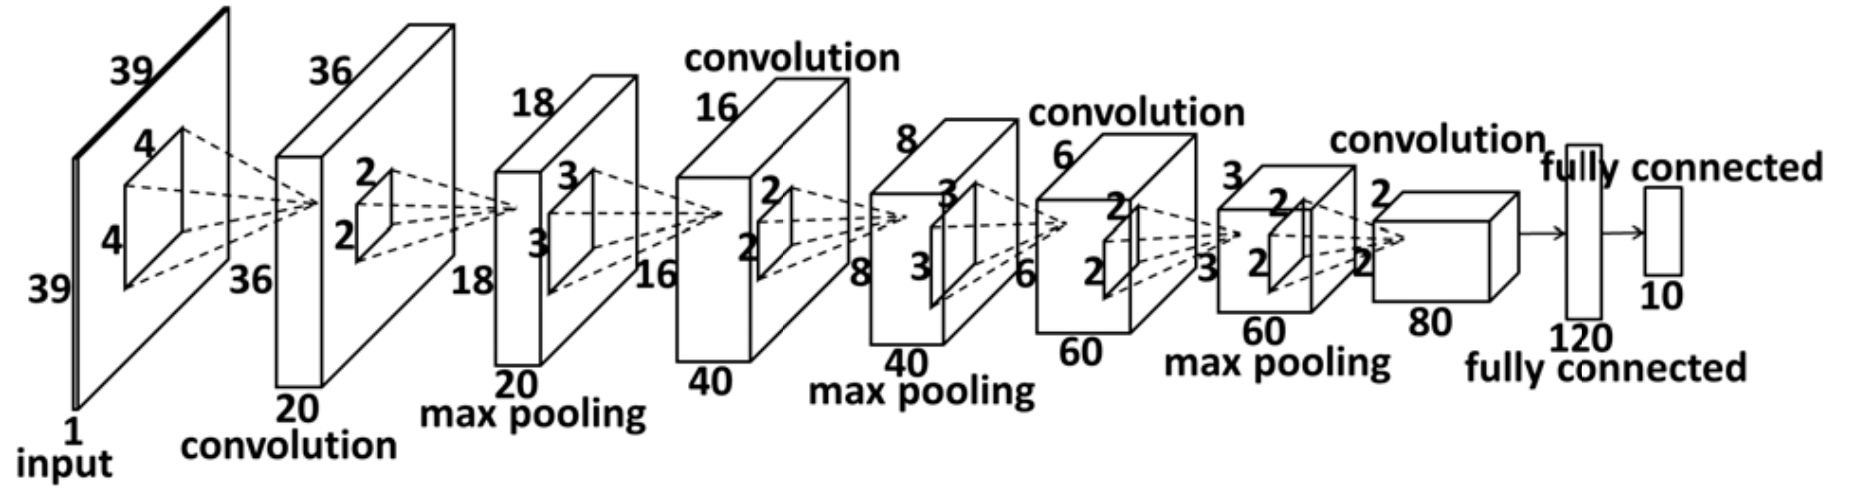
\includegraphics[width=\hsize]{figures/cnn.png}
  \caption{畳み込みニューラルネットワークの例\cite{sun2013deep}}
  \label{fig:cnn}
\end{figure*}

\subsection{spectral convolution}
spectral convolution\cite{bruna2013spectral}はグラフにおける信号処理の考え方\cite{Shuman2013signal_processing_graph}に基づいてグラフ上で畳み込み演算を定義する手法である。この手法はまずグラフ上のデータをグラフラプラシアンの固有値分解を用いて信号の傾きにより成分分解し、求められた要素積を逆フーリエ変換によりノードの情報を更新する手法である。図\ref{fig:spectral}ではこの手法をグラフに適用した例を示している。

しかしこの手法には
\begin{itemize}
	\item 固有値分解の計算量が大きい
	\item グラフ上では空間的に局在化されたフィルターを得ることができない
    \item セルフループや多重エッジに適用できない
\end{itemize}
などの問題がある。

\vspace{1cm}

\begin{figure*}[tb]
  \centering
  \includegraphics[width=0.5\hsize]{figures/filtering.eps}
  \caption{spectral convolution\cite{bruna2013spectral}}
  \label{fig:spectral}
\end{figure*}

\subsection{spatial convolution}

spatial convolution\cite{gilmer2017neural}はspectral convolutionの問題点である計算量が大きいことやセルフループや多重辺を持つグラフに適用できない問題点を解決した手法である。この手法ではグラフ構造の近隣ノードの信号の情報を用いて自身のノードの情報を更新していくことにより畳み込みを定義する。ノード$i$における畳み込み演算は以下の式で表せる。

\begin{equation}
\displaystyle h^{(l+1)}_i = \sigma \left(h^{(l)}_i W^{(l)}_0 + \sum_{j \in {N_i}} \frac{1}{c_{i, j}} h^{(l)}_j W^{(l)}_1  \right).
\end{equation}

ここで$N_i$はノード$i$にエッジを張るノードの集合であり、$c_{i,j}$は正規化のための定数である。また$W^{(l)}_0$、$W^{(l)}_1$は第$l$層における隠れ層の重み行列である。

\begin{figure*}[tb]
  \centering
  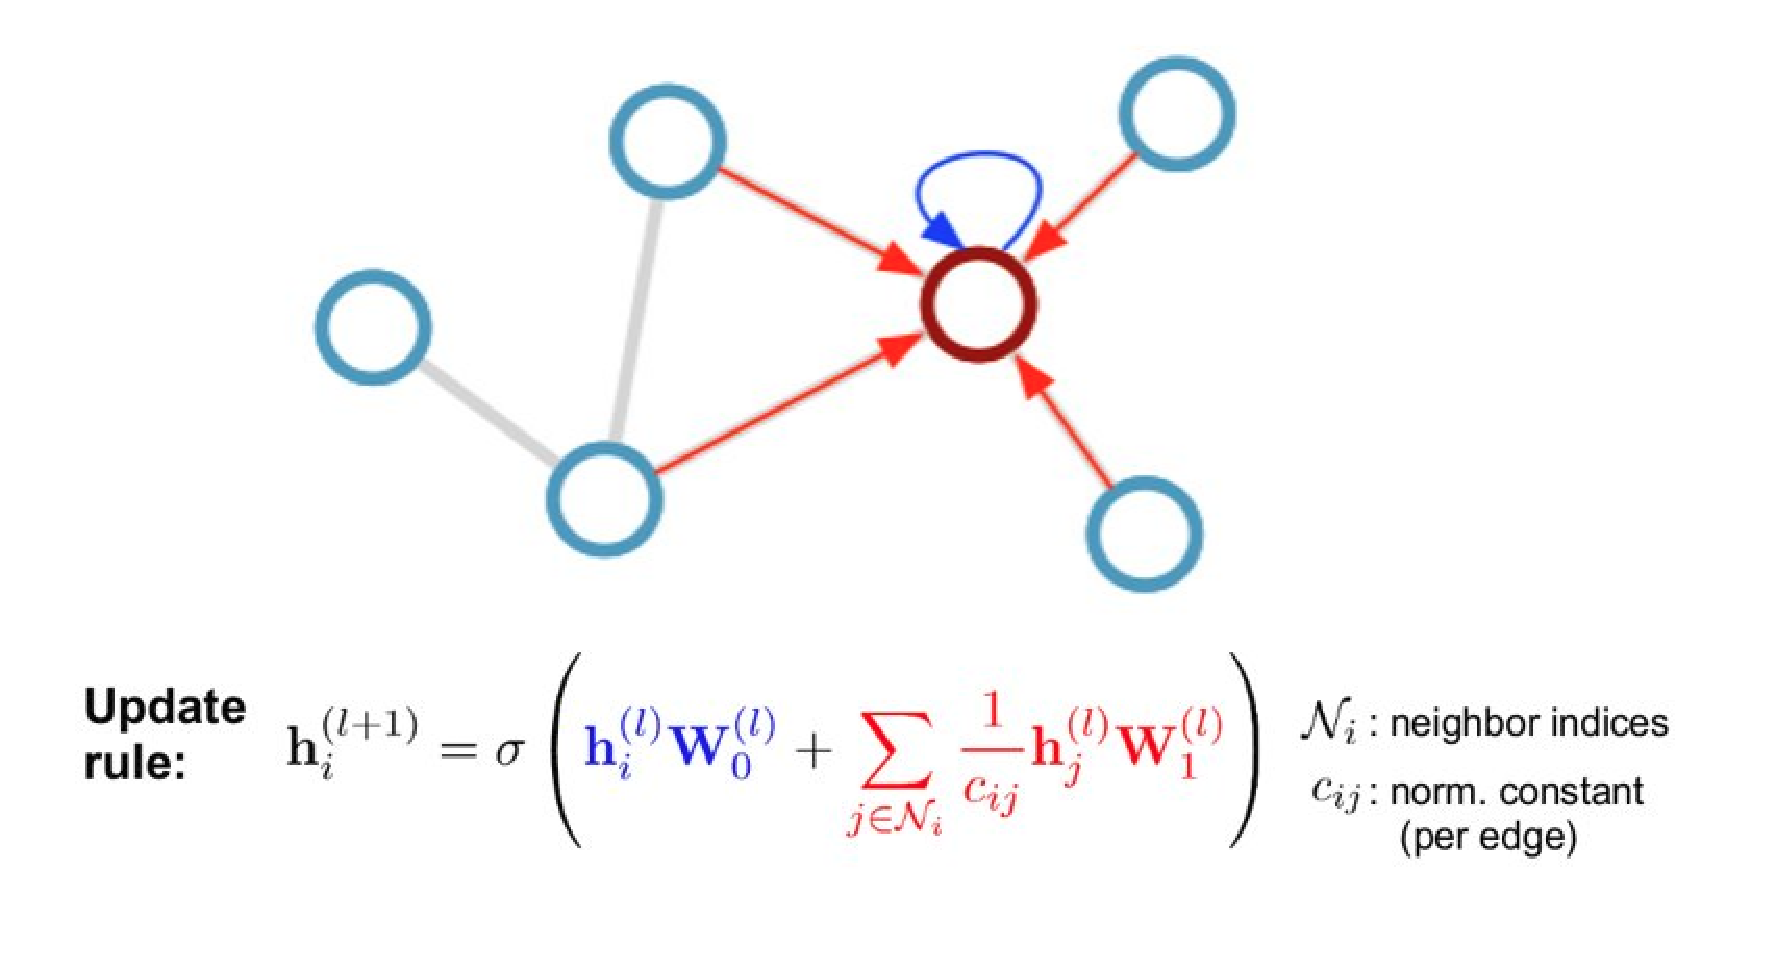
\includegraphics[width=0.7\hsize]{figures/spatial.eps}
  \caption{spatial convolution\cite{kipf2016GCN}}
  \label{fig:spatial}
\end{figure*}

\section{グラフ畳み込みネットワーク}
グラフ畳み込みネットワーク(Graph Convolutional Network;GCN)\cite{kipf2016GCN}はspactral convolution を spatial convolutionとしても解釈できることを示した手法である。
グラフ畳み込みネットワークの第$i$層の出力は以下の式で表せる。
\begin{equation}
H^{(i)} = \sigma(D^{-1/2}\tilde{A}D^{-1/2}H^{(i-1)}W^{(i)})
\end{equation}

ここで、$I_{n}\in \mathcal{R}^{n \times n}$は単位行列、$\tilde{A}=A+I_{n}$、$D \in \mathcal{R}^{n \times n}$は次数行列、$H^{(0)}=X$、$W^{(i)}$は$i$層における特徴行列を更新するための重み行列である。また、$\sigma$はReLU関数やsigmoid関数などの活性化関数である。

GCNと同様にグラフ上で畳み込み演算をする手法として、エッジにAttention\citation{vaswani2017attention}をかけて学習するGAT\cite{velivckovic2017GAT}や、Mean AggregatorやLSTM Aggregatorなどを用いたGraphSAGE\cite{hamilton2017GraphSAGE}、weisfeiler-lehmanテストを用いたGIN \cite{xu2018how_powerful_gnn}、Mix-hop-propagationを用いるMixHop\cite{sami2019mixhop}といった手法が後に提案された。

GCNは層を重ねるごとにノードの情報量が指数関数的に喪失するoversmoothingが発生するため一般的には2層GCNが用いられるが\cite{li2018deeper}、oversmoothingを回避するための手法\cite{luan2019break,chenWHDL2020gcnii}が近年提案された。またノード数が数億を超える大きいグラフに対応させるためにGCNの計算量を削減するためにサンプリングを用いた手法\cite{hamilton2017GraphSAGE, chen2018fastgcn}やバッチ学習を行う手法\cite{chiang2019cluster}も提案されている。

\subsection{半教師ありノード分類}
GCNを用いて半教師ありノード分類するタスクにおいては、一般的にグラフ$\mathcal{G} = (\mathcal{V}, \mathcal{E})$を表す隣接行列$\mathbf{A}$とノード特徴量$\mathbf{X}$、一部ノードのラベル$\boldsymbol{y}_{train} \in \mathcal{Y}$を入力データとして、ラベルの与えられていない残りのノードのラベル$\mathcal{Y}$を予測する精度を測る。

GCNは一般的には2層用いられ、2層GCNは以下の式で表せる。

\begin{align}
    \label{eq:gcn_nodecls}
    \hat{\mathbf{Y}} = \mathrm{GCN}(\mathbf{X}, \mathbf{A}) \coloneqq \softmax (\hat{\mathbf{A}} \relu (\hat{\mathbf{A}} \mathbf{X} \mathbf{W}^{(1)})\mathbf{W}^{(2)})
\end{align}

ここで$\hat{\mathbf{Y}} = [\hat{\boldsymbol{y}}_1, \dots, \hat{\boldsymbol{y}}_N]^{\mathsf{T}} \in [0, 1]^{N \times C}$はノードのラベル予測を行列で表している。またGCNはノードごとに$\hat{\boldsymbol{y}}_i = [\hat{y}_{i1}, \dots, \hat{y}_{iC}]^{\mathsf{T}}$の出力によりそれぞれのノードのラベルの予測を行列で示している。ここで$0 \leq \hat{y}_{ic} \leq 1$かつ$\sum_c \hat{y}_{ic} = 1$という制約の中で$\hat{y}_{ic}$は、ノード$i$がクラス$c$に属する確率を表す。


他クラス分類においては、交差エントロピー誤差を用いることで学習の損失関数は以下のように計算できる。

\begin{equation}
L_{supervised} = - \sum_{i \in \mathcal{V}_{train}} \sum_{c=1}^C y_{ic} \log \hat{y}_{ic}
\end{equation}
ここで$\boldsymbol{y}_i \in \{0,1\}^C$はラベル付けされたノードの場合1、それ以外で0で表されるようなone-hotベクトルを用いて各ノードの正解ラベルを表す。

\subsection{リンク予測}
リンク予測は一般的にはグラフ$\mathcal{G} = (\mathcal{V}, \mathcal{E}_{train})$を表す隣接行列$\mathbf{A}_{train}$、ノード特徴量$\mathbf{X}$を用いて、情報が与えられていない2ノード間のエッジの有無を予測するタスクである。ここで$\mathcal{E}_{train}$は完全データからエッジの教師データのみを抽出した集合である。

GCNを用いてリンク予測を行うモデルとして提案手法で用いるVGAE\cite{kipf2016variational}について述べる。VGAEは変分オートエンコーダ(Variational Auto Encoder;VAE)\cite{kingma2013auto}をグラフに適用したモデルである。

VGAEはエンコーダとデコーダから構成される。エンコーダではGCNを用いてノードの特徴量と隣接行列から確率的な潜在表現を学習し、デコーダでは内積とシグモイド関数を用いて元の隣接行列を復元する。

まずエンコーダについて述べる。本章では2層エンコーダを用いた計算について記す。まず確率変数$\boldsymbol{z}_i \in \mathbb{R}^{F}$を用いて平均$\boldsymbol{\mu}_i \in \mathbb{R}^{F}$と対角共分散行列$\diag(\boldsymbol{\sigma}_i) \in \mathbb{R}^{F \times F}$は以下の式で計算できる。

\begin{align}
    [\boldsymbol{\mu}_1, \dots, \boldsymbol{\mu}_N] &= \mathrm{GCN}_{\boldsymbol{\mu}}(\mathbf{X}, \mathbf{A}) \coloneqq \hat{\mathbf{A}} \relu (\hat{\mathbf{A}} \mathbf{X} \mathbf{W}^{(1)})\mathbf{W}_{\boldsymbol{\mu}}^{(2)} \label{eq:vgae_encoder_mu}\\
    [\boldsymbol{\sigma}_1, \dots, \boldsymbol{\sigma}_N] &= \mathrm{GCN}_{\boldsymbol{\sigma}}(\mathbf{X}, \mathbf{A}) \coloneqq \hat{\mathbf{A}} \relu (\hat{\mathbf{A}} \mathbf{X} \mathbf{W}^{(1)})\mathbf{W}_{\boldsymbol{\sigma}}^{(2)} \label{eq:vgae_encoder_sigma}
\end{align}

ここで$\mathrm{GCN}_{\boldsymbol{\mu}}$と$\mathrm{GCN}_{\boldsymbol{\sigma}}$の計算においてGCN1層目に用いる重みパラメータ$\mathbf{W}^{(1)}$を共有している。また確率変数$\boldsymbol{z}_i \in \mathbb{R}^{F}$と求められた平均平均$\boldsymbol{\mu}_i \in \mathbb{R}^{F}$と対角共分散行列$\diag(\boldsymbol{\sigma}_i) \in \mathbb{R}^{F \times F}$を用いるとエンコーダは以下の式で計算できる。

\begin{align}
  q(\mathbf{Z} | \mathbf{X}, \mathbf{A}) &= \prod_{i=1}^N q(\boldsymbol{z}_i | \mathbf{X}, \mathbf{A})\\
  &= \prod_{i=1}^N \mathcal{N} (\boldsymbol{z}_i | \boldsymbol{\mu}_i, \diag(\boldsymbol{\sigma}_i^2)) \label{eq:vgae_encoder_output}
\end{align}




次にデコーダについて述べる。デコーダはノードペアの潜在変数の内積により隣接行列を復元する。
\begin{align}
    p(\mathbf{A} | \mathbf{Z}) &= \prod_{i=1}^N \prod_{j=1}^N p(A_{ij} | \boldsymbol{z}_i, \boldsymbol{z}_j)
\end{align}
ここで$p(A_{ij} = 1 | \boldsymbol{z}_i, \boldsymbol{z}_j) = \sigmoid(\boldsymbol{z}_i^{\mathsf{T}} \boldsymbol{z}_j)$とすることで$\boldsymbol{z}_i$と$\boldsymbol{z}_j$の内積がエッジの存在確率を表すようにしている。

最後に損失関数について述べる。潜在変数の事前分布を$p(\mathbf{Z}) = \prod_i p(\boldsymbol{z}_i) = \mathcal{N}(\boldsymbol{z}_i | \boldsymbol{0}, \mathbf{I})$、潜在変数を$\boldsymbol{z}_i = \boldsymbol{\mu}_i + \boldsymbol{\epsilon}\odot \boldsymbol{\sigma}_i$(ノイズを$\boldsymbol{\epsilon} \sim \mathcal{N}(\boldsymbol{0}, \mathbf{I})$、要素積を$\odot$として表す)とすると損失関数は以下の式で表せる。

\begin{align}
    \mathcal{L} &= \mathbb{E}_{q(\mathbf{Z} | \mathbf{X}, \mathbf{A})}[\log p(\mathbf{A} | \mathbf{Z})] - \mathrm{KL}[q(\mathbf{Z} | \mathbf{X}, \mathbf{A}) || p(\mathbf{Z})]
\end{align}

隣接行列$p(\mathbf{A})$を直接求めるためには計算量的に困難であるため、変分下限を最大化する目的関数を用いている。


\section{欠損データ}
\subsection{実世界上の欠損値}
\begin{figure*}[tb]
  \centering
  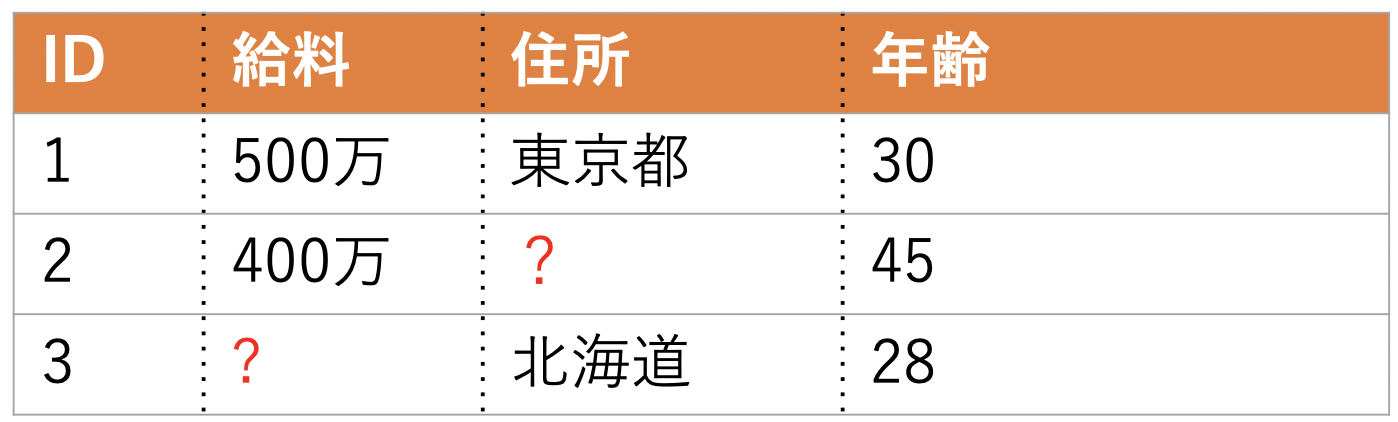
\includegraphics[width=0.5\hsize]{figures/missing_example.png}
  \caption{欠損値の例(ユーザー情報)}
  \label{fig:missing_example}
\end{figure*}
実世界において欠損値を含むデータは数多く存在する。
\begin{itemize}
	\item 人的なミス
	\item センサーによるエラー入力
	\item 任意回答における未入力項目を含むアンケート
    \item ビッグデータの情報欠損
\end{itemize}
このような欠損値を含むデータ構造は図\ref{fig:missing_example}のようなデータとして保持される。

\subsection{欠損値のパターンと表現}
\begin{figure*}[tb]
  \centering
  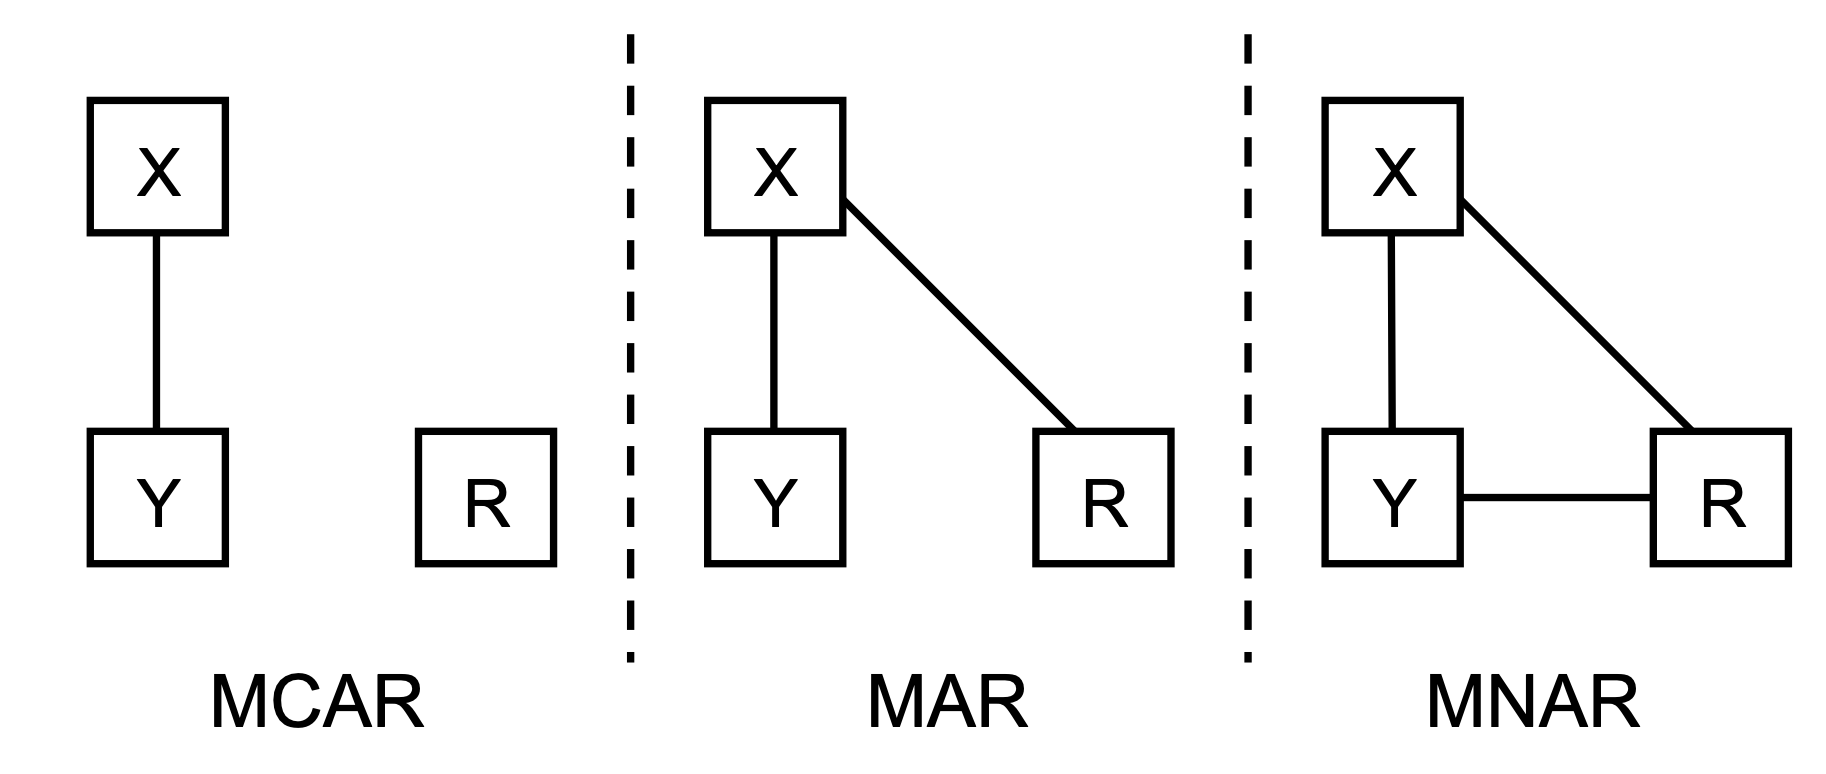
\includegraphics[width=\hsize]{figures/missing_pattern.png}
  \caption{欠損パターンの概念図。Rを欠損識別変数、Xを観測値データ、Yを欠損値データとして表している。}
  \label{fig:missing_pattern}
\end{figure*}
データ中の一部の値が不明のデータは一般に欠損データ(missing data)と呼ばれる。欠損データは値が分かる観測値(observed value)と値が不明の欠損値(missing value)から構成される。欠損値を一つも含まないデータは完全データ(complete data)と呼ばれ、欠損値を1つでも含むデータを不完全データ(incomplete data)と呼ばれている。

$R$を欠損識別変数、$X_o$を観測値データ、$X_m$を欠損値データとすると、ある特徴量が欠損している確率は条件付き確率を用いて$p(\mathbf{R}| \mathbf{X}_{o}, \mathbf{X}_{m})$と表すことができる。また、Littleらによると欠損値のパターンは3つに分類することができる\cite{little2019statistical}。
\begin{itemize}
    \item MCAR (Missing Completely At Random):\\
    MCARはデータ構造に関係なく、欠損値となるデータが完全にランダムに決定されたケースである。条件付確率は$p(\mathbf{R}| \mathbf{X}_{o}, \mathbf{X}_{m}) = p(\mathbf{R})$と表現できる。図\ref{fig:missing_pattern}の左図はMCARの概念図である。
    \item MAR (Missing At Random):\\
    MARはデータの欠損している確率がそのデータの種類により決定されたケースである。そのためMARはMCARよりも制約が弱く、MARはMCARをより抽象化したケースと言える。条件付確率は$p(\mathbf{R}| \mathbf{X}_{o}, \mathbf{X}_{m}) = p(\mathbf{R}| \mathbf{X}_{obs})$と表現できる。図\ref{fig:missing_pattern}の中央図はMARの概念図である。
    \item MNAR (Missing Not At Random):\\
    MNARは欠損値を持つ変数がそれぞれの欠損値の有無により決定されるケースである。条件付確率は$p(\mathbf{R}| \mathbf{X}_{o}, \mathbf{X}_{m}) \neq p(\mathbf{R}| \mathbf{X}_{obs})$と表現できる。図\ref{fig:missing_pattern}の右図はMNARの概念図である。
\end{itemize}

これらの欠損値のパターンではMCAR、MAR、MNARの順番で扱いやすい一方、現実世界の複雑性から、欠損値を含む実データの多くはMNARであることが知られている。

\section{欠損値補完}
欠損値を扱う方法は以下の3つに分類することができる。
\begin{itemize}
\item 欠損値の除去 
\item 代入法(imputation)
\item 不完全データとして扱う
\end{itemize}
\subsection{欠損値の除去}
欠損値の除去は欠損値を含む項目をデータセットから取り除く手法である。欠損値を除去する方法はリストワイズ除去とペアワイズ除去の2種類がある。図\ref{fig:missing_delete}は不完全データ(a)に対する欠損値除去の例を(b)、(c)で示している。(b)のリストワイズ除去\cite{GarciaLaencina2010}は解析対象の持つ変数のうちどれか一つでも欠損値を持つケースのデータを削除する方法である。この手法は欠損率が高い場合に情報量がとても小さくなってしまう問題がある。(c)のペアワイズ除去は変数のうちどれか一つでも欠損値を持つケースのデータを選択的に削除する方法である。リストワイズ除去と比べて情報を多く保持できる一方、欠損値を含むためデータが扱いづらい問題がある。

\begin{figure*}[tb]
  \centering
  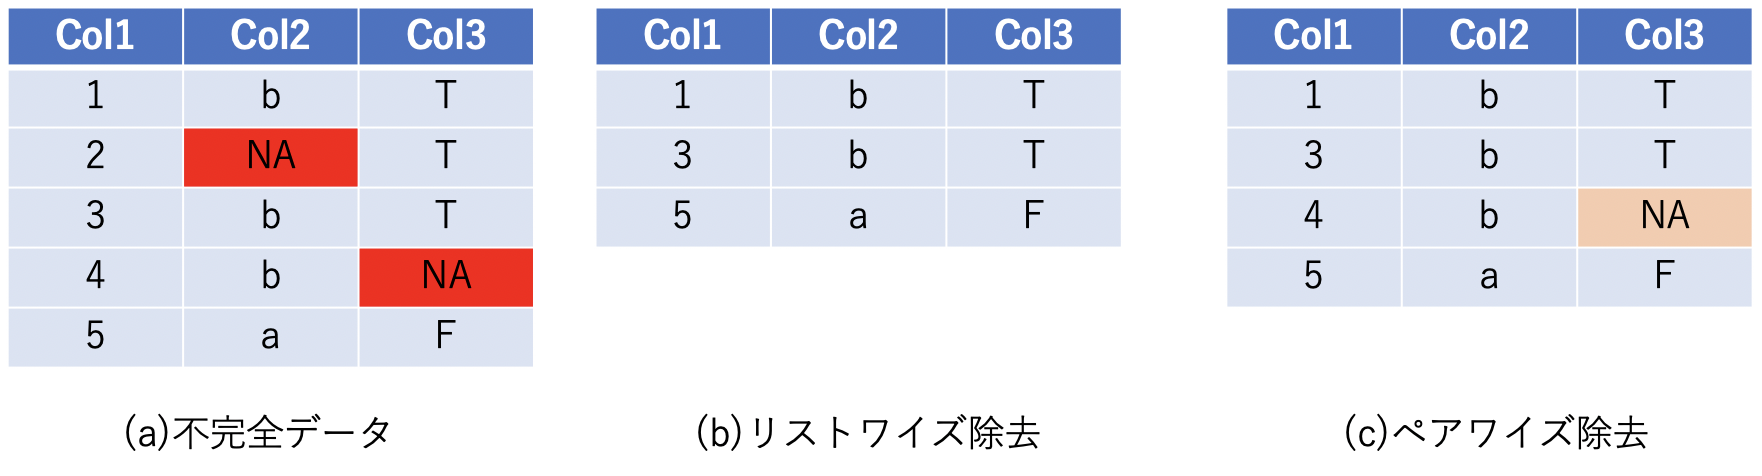
\includegraphics[width=1\hsize]{figures/missing_delete.png}
  \caption{欠損値の除去の例}
  \label{fig:missing_delete}
\end{figure*}

\subsection{代入法(imputation)}
代入法とは欠損値を何らかの方法を用いて補完することで不完全データを完全データにする方法である。図\ref{fig:missing_imputation}は代入法を用いて不完全データ(a)を完全データ(b)に変換している。ここで$X_{ij}$は定数である。代入法は完全データが得られるため、得られたデータに既存の機械学習手法を適用することができるという強みがある一方、誤った欠損値補完をすることで精度を下げてしまう可能性があるという問題がある。

\subsection{不完全データとして扱う}
欠損値をもつ不完全データをそのまま扱う手法がある。この場合は観測値の情報を欠損なしで扱うことができ、また代入法とは異なり誤ったデータを用いることなく解析することができるが、データに欠損値を含むためデータの扱いが難しいという問題がある。GMMC\cite{smieja2018GMMC}を用いて学習する手法\cite{taguchi2021graph}やアンサンブル学習を用いた手法\cite{jiang2005ensemble}、オートエンコーダを用いた手法\cite{Smieja2019}などがある。

\begin{figure*}[tb]
  \centering
  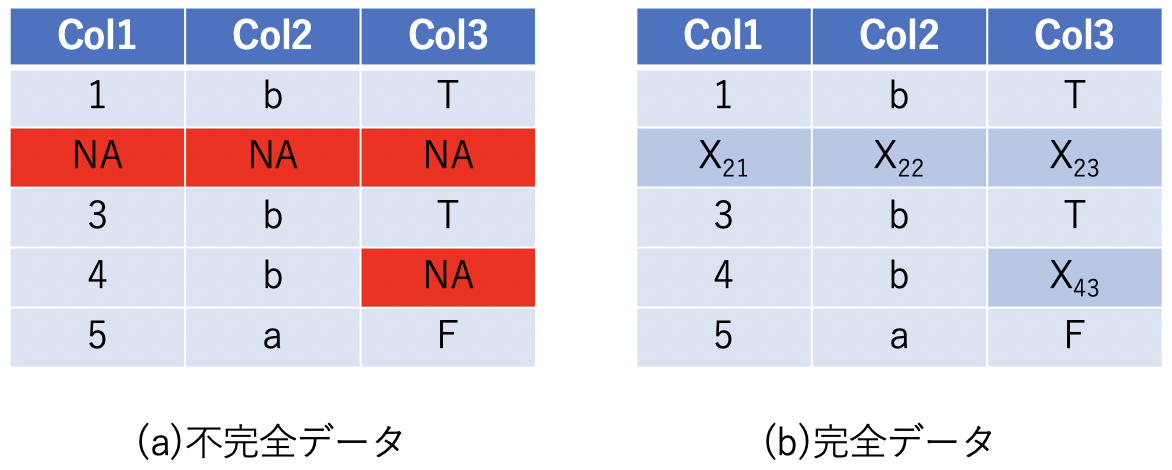
\includegraphics[width=0.7\hsize]{figures/missing_imputation.png}
  \caption{代入法(imputation)の例}
  \label{fig:missing_imputation}
\end{figure*}


